\documentclass[12pt]{article}

\usepackage[margin=3cm]{geometry}
\usepackage{graphicx}
\usepackage{amsmath}
\usepackage{natbib}
\usepackage{hyperref}
\bibliographystyle{apalike}

\begin{document}

\section{Simple example: 90th US Senate roll call data}

To exemplify the use of the EPC-interest using a relatively simple latent variable model with categorical variables that is well-known in political science, we estimate an ideal point model on roll call data \citep{jackman2010pscl} for senators in the 90th US Senate, which met from 1967 to 1969 during the Lyndon B. Johnson Administration. 

The probability that senator $i$ votes ``Yea'' on motion $j$ is modeled as a logistic regression on the motion's (unobserved) utility, 
\begin{equation}
	P(\text{``Yea'' on motion } j | x_i) = [1 + \exp(-\beta_j u_{ij})]^{-1},
	\label{eq:vote-nodif}
\end{equation}
where the utility $u_{ij}$ of the motion to that senator is simply the Euclidean distance between the senator's position $x_i$ and the motion's position $\tau_j$,
\begin{equation}
	u_{ij} = (x_{i} - \tau_{j})^2.
\end{equation}
The latent variable $x_i$ is known in the literature as an ``ideal point''. This model is equivalent to the well-known unidimensional \citet{poole1985spatial} (W-NOMINATE) model, and can be estimated in specialized software \citep[e.g.][]{poole2008scaling} or by software capable of  factor analysis with quadratic factors \citep{maraun2001extra}. 


The Poole-Rosenthal model can be extended to incorporate covariates that predict the latent variable $x_i$, for example using the party of the senator as a predictor: 
\begin{equation}
	x_i = \alpha + \gamma \cdot \text{Party} + \epsilon_i.
	\label{eq:party-dimension}
\end{equation}
Using party (Democratic or Republican) as a predictor allows the researcher to see how strongly  party membership relates to the senator's ideological position, which ultimately influences their votes. A higher value of $\gamma$ thus indicates more ideological homogeneity  within parties in the Senate: we therefore call $\gamma$ the ``polarization coefficient''.  

The usual choice $\epsilon_i \sim \text{Normal}(0, \sigma^2)$  leads to a quadratic structural equation model (SEM) for categorical data, or, equivalently, a quadratic 2PL IRT model with a covariate \citep{rabe2004generalized}. Alternatively, the distribution of $x$ can be estimated from the data by choosing some number $K$ of categories for $x$ (``latent classes'') and modeling the probability of belong to class $k$ as an ordered multinomial regression,
\begin{equation}
	P(x_i = k | \text{Party}) = \frac{\exp(\alpha_k + \gamma \cdot x^{(k)} \cdot \text{Party})}
		{\sum^{K}_{m=1} \exp(\alpha_m + \gamma \cdot x^{(m)} \cdot \text{Party})},
\end{equation}
where $x^{(m)}$ is a latent score assigned to the $k$-th category of $x$. For this arbitrary choice of latent scale, we choose $x^{(m)}$ to go from 0 to 1 in equally spaced intervals \citep[following][]{vermunt2013technical}. The latent category intercepts $\alpha_k$ allow the distribution of the latent dimension to be freely estimated rather than assumed Normal. This leads to the ``latent class factor model'' \citep{vermunt_factor_2004}, for which the Likelihood is 
\begin{equation}
	P(\text{Voting pattern of senator } i) = \sum^{K}_{m=1} P(x_i = m) 
	\prod^{J}_{j=1} P(\text{Senator's vote on motion } j| x_i).
\end{equation}


%In familiar techniques such as W-NOMINATE or Optimal Classification Roll Call Scaling \citep{Poole:2005aa}, investigating the relationship of the latent dimension $x_i$ with external variables is often accomplished by first estimating the ideal point estimates $\hat{x}_i$ and then correlating or plotting these values with the covariate. The current formulation 	\label{eq:party-dimension} attains the same goal in one step, with the possible advantage that measurement error in the ideal point estimates is accounted for in the estimation of the polarization coefficient of interest $\gamma$.

A possible problem when using ideal point models to investigate polarization is that it is assumed that this polarization is the same on all motions the Senate votes on. If there is some motion on which the votes of senators from the same party are significantly more tight-knitted than usual, there will be an effect of Party over and above that of the senator's utility for this motion. A vote model with a direct covariate effect,
\begin{equation}
		P(\text{``Yea'' on motion } j | x_i) = [1 + \exp(-\beta_j u_{ij} - \delta_j \cdot\text{Party})]^{-1},
	\label{eq:vote-dif}
\end{equation}
then replaces Equation \ref{eq:vote-nodif}. In other words, the usual ideal point model assumes measurement invariance with respect to the covariates, an assumption that can be expressed as $\delta_j=0$. In the current application, where such direct effects do exist they are relevant to the investigation of polarization insofar as ignoring them biases the estimate of the Senate's overall polarization. Thus, we investigate whether the assumption of measurement invariance $\delta_j=0$  seriously affects the estimate of interest $\hat{\gamma}$ using the EPC-interest.

Maximum likelihood estimates of the parameters were obtained using Latent Gold, taking $K=4$ and the first 20 motions introduced in the 90th Senate as an example. The model appears to fit the data well, with an $L^2$ bootstrapped $p$-value of $0.14$, The factor scores $\hat{x}_i$ obtained from this simple model correlated highly (0.79) with those obtained from W-NOMINATE \citep{poole2008scaling} and from Optimal Classification Roll Call Scaling \citep[0.81;][]{poole2012oc}.
Based on the full invariance model, the polarization coefficient $\hat{\gamma}$ was estimated at $4.164$ (s.e. 1.3077). Since $\gamma$ is a logistic regression coefficient, this means that a Republican senator has a $\exp(\hat{\gamma})=\exp(4.164)\approx64$ times higher odds of being one category above a Democratic senator than of being in the same category. There was therefore considerable polarization in the 90th Senate. 

However, violations of measurement invariance could conceivably bias this conclusion. To investigate this, Figure \ref{fig:epc-interest} plots the EPC-interest values of freeing the direct effects $\delta_j$ on the parameter estimate of interest $\hat{\gamma}$. Each number in Figure \ref{fig:epc-interest} corresponds to a motion number introduced in the Senate. The vertical axis, labeled ``EPC-interest'', estimates the change from the current estimate (4.164) under full measurement invariance that one can expect to observe in $\hat{\gamma}$ when freeing the direct effect of Party for that motion. 
The horizontal axis shows the $p$-value for the null hypothesis that the corresponding $\delta_j = 0$, adjusted for false discovery rate \citep{benjamini1995controlling}. The idea behind plotting both of these quantities at the same time is that the researcher will likely be interested in violations of measurement invariance that are both statistically and substantively significant \citep{saris2009testing}.

\begin{figure}\centering
\includegraphics[width=.9\textwidth]{../../outputs/EPC-interest.pdf}
\caption{The effect of twenty measurement invariance assumptions on the polarization parameter of interest $\gamma$, plotted against the p-values for each violation.}
\label{fig:epc-interest}
\end{figure}

Figure \ref{fig:epc-interest} shows that, of the statistically significant violations of measurement invariance, motion \#03 violates measurement invariance in a manner that augments the estimated polarization (EPC-interest is positive). Motions \#04 and \#13, violate measurement invariance in an approximately opposite manner (EPC-interests are negative). However, one motion, \#20, clearly stands out as an important violation of measurement invariance.
After introducing the direct effect of party on voting ``Yea'' to Motion \#20 (freeing $\delta_{20}$), no other measurement invariance violations are statistically significant (all false discovery rate-adjusted $p$-values $\geq 0.05$). Thus, it seems that Motion \#20 (HR4573, which increased the public debt limit) was an issue on which the ranks were closed more than usual. Indeed, the 1967 CQ Almanac\footnote{\url{http://library.cqpress.com/cqalmanac/document.php?id=cqal67-1314297}} specifically reports on this motion, remarking that ``Republicans launched their first major attacks in the 90th Congress on the Administration's fiscal policies'', with no Republicans voting in favor. 

After adjusting for this event, the polarization coefficient is estimated at 3.422 (s.e. 1.0630): the tight-knittedness between party membership and voting pattern is therefore somewhat loosened, but still strong.  The partial invariance model after accounting for this one violation becomes acceptable, in  the sense that those violations that are present do not substantially change the results of interest regarding polarization. The model fit the data well with an $L^2$ bootstrapped $p$-value of $0.11$. Its BIC (1379) indicates an improvement over that of the full invariance model (1405).  Overall, the difference between the fully and partially invariant models are modest. Figure \ref{fig:ideal-points} shows the effect of freeing $\delta_{20}$ on the ``ideal point'' estimates, i.e. the latent variable estimates $\hat{x}_i$. 

\begin{figure}\centering
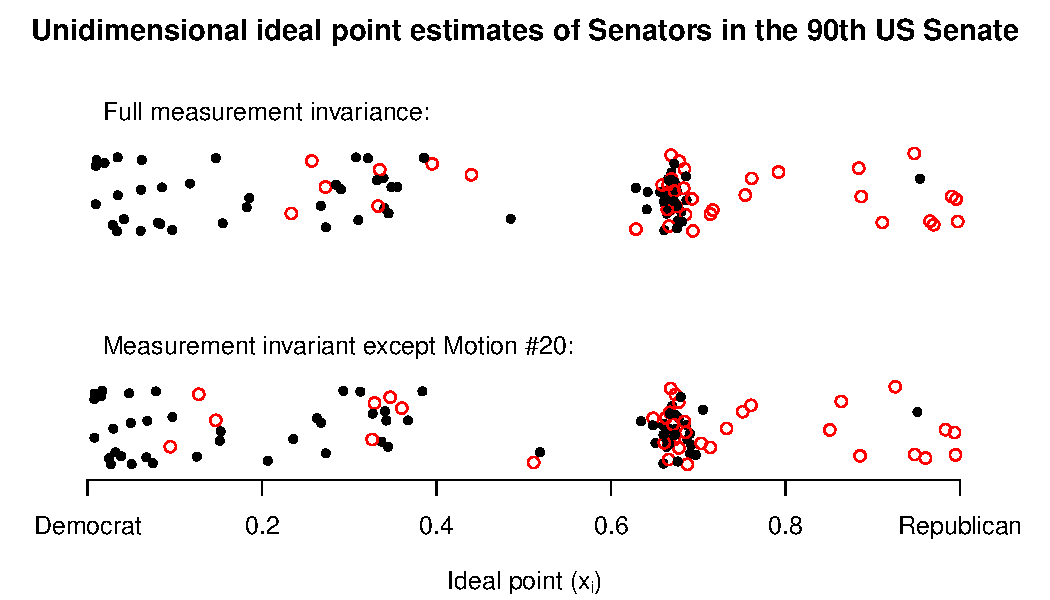
\includegraphics[width=.9\textwidth]{../../outputs/ideal-points.pdf}
\caption{Posterior point estimates of the latent variable ``ideal point'' score $\hat{x}_i$ for all senators (points), jittered vertically for visual clarity. Black points are Democrats, red circles Republicans. Top: estimates under the fully invariant model; Bottom: estimates allowing for the direct effect $\delta_{20}\neq0$.}
\label{fig:ideal-points}
\end{figure}

The top part of Figure \ref{fig:ideal-points} shows the ideal point estimates under the full invariance model. These estimates range from zero to one; since Democrats, shown as black dots, are predominantly on the lower side of the scale, zero has been labeled ``Democrat'' and the score 1 has been labeled ``Republican'', since most Republicans (red circles) can be found here. To make the points more visible, they have been jittered randomly in the vertical direction. The bottom part of Figure \ref{fig:ideal-points} shows the ideal point estimates for the same senators, but this time while accounting for the partial violation of measurement invariance $\delta_{20}\neq0$. It can be seen that Republicans  are more spread out into the ``Democratic'' side of the scale. Especially the three Republican senators with a score below 0.2 experience a rather large shift in position. On the whole, therefore, the differences between the two distributions are modest, but the differences for individual senators' ideal point estimates can be quite substantial.

\bigskip
In this section we investigated measurement invariance assumptions in the well-known ``ideal point'' model for example binary roll call data. The  example  demonstrated that even when the model appears to fit the data well initially, it is still possible for violations of measurement invariance to bias the conclusions. The EPC-interest was used here as a tool to detect such bias. After accounting for one violation of measurement invariance, the final model differed somewhat from the original conclusions: the estimated amount of polarization in the 90th Senate was lower and several Republican senators' estimated ideological positions were considerably more liberal. 




\bibliography{/Users/daob/Dropbox/Bibliography/quality}
\end{document}